
\section*{Постановка задачи}
Разработать программу для рассылки новостей подписчикам. 
Реализовать доставку сообщений через протокол TCP/IP. 
Использовать события для отображения подписки и отписки подписчиков на серверной стороне приложения.
Клиентская часть приложения может присоединится и отсоединится к серверу, читать новости, которые отсылает сервер.

Описать модель клиент-сервер.

Описать шаблон проектирования Наблюдатель, который будет реализован в приложении для отображения связи один-ко-многим.

Сделать код данного проекта доступным всему человечеству: \url{https://github.com/tstuteam/NewsDistribution}.
\addcontentsline{toc}{section}{Постановка задачи}

\newpage
\section{Модель клиент–сервер}

\textbf{Модель клиент - сервер} - вычислительная или сетевая архитектура, в которой задания или сетевая нагрузка распределены между поставщиками услуг, называемыми серверами, и заказчиками услуг, называемыми клиентами.
Часто клиенты и серверы взаимодействуют по компьютерной сети на отдельном оборудовании, но и клиент, и сервер могут находиться в одной и той же системе. 
Серверный узел запускает одну или несколько серверных программ, которые совместно используют свои ресурсы с клиентами.
Клиент обычно не предоставляет общий доступ ни к одному из своих ресурсов, но он запрашивает контент или услугу с сервера.
Таким образом, клиенты инициируют сеансы связи с серверами, которые ожидают входящих запросов.
Примерами компьютерных приложений, использующих модель клиент-сервер, являются электронная почта, сетевая печать и Всемирная паутина.

\begin{figure}[H]
	\begin{center}
		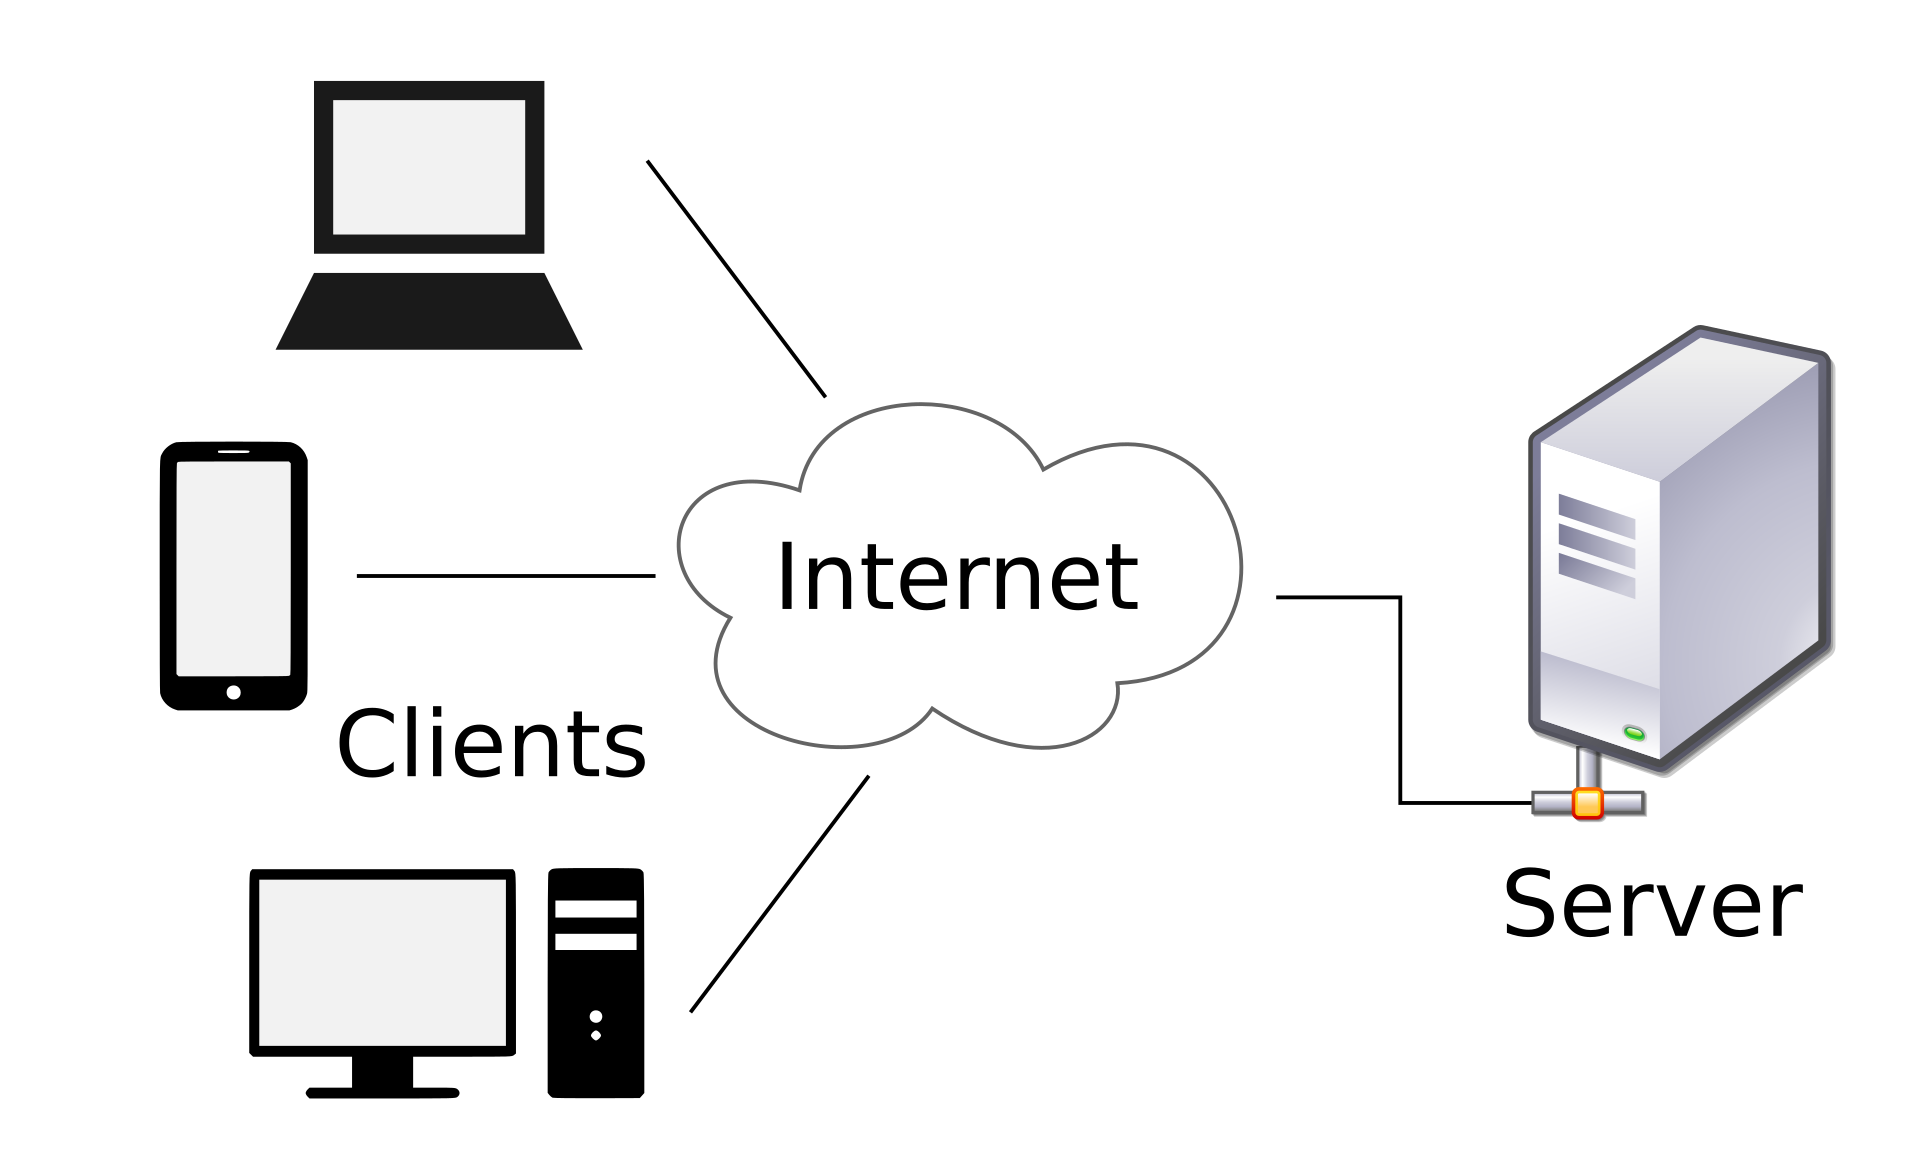
\includegraphics[width=\textwidth]{1920px-Client-server-model.svg.png}
		\caption{Схема компьютерной сети клиентов, общающихся с сервером через Интернет.}
	\end{center}
\end{figure}

\subsection{Роль клиента и сервера}

Характеристика "клиент-сервер" описывает отношения взаимодействующих программ в приложении.
Серверный компонент предоставляет функцию или услугу одному или нескольким клиентам, которые инициируют запросы на такие услуги.
Серверы классифицируются по услугам, которые они предоставляют.
Например, веб-сервер обслуживает веб-страницы, а файловый сервер обслуживает компьютерные файлы.
Совместно используемым ресурсом может быть любое программное обеспечение и электронные компоненты серверного компьютера: от программ и данных до процессоров и устройств хранения.
Совместное использование ресурсов сервера является \textit{услугой, сервисом} (service).

Является ли компьютер клиентом, сервером или и тем, и другим, определяется характером приложения, которому требуются сервисные функции.
Например, на одном компьютере могут одновременно работать веб-сервер и программное обеспечение файлового сервера, чтобы предоставлять разные данные клиентам, выполняющим разные виды запросов.
Клиентское программное обеспечение также может взаимодействовать с серверным программным обеспечением на том же компьютере.
Связь между серверами, например для синхронизации данных, иногда называется \textit{межсерверной связью} или связью \textit{сервер-сервер}.

\subsection{Взаимодействие клиента и сервера}

Как правило, сервис представляет собой абстракцию компьютерных ресурсов, и клиенту не нужно беспокоиться о том, как работает сервер при выполнении запроса и доставке ответа.
Клиенту нужно только понять ответ на основе известного прикладного протокола, т. е. содержание и форматирование данных для запрошенной услуги.

Клиенты и серверы обмениваются сообщениями по шаблону обмена сообщениями запрос-ответ.
Клиент отправляет запрос, а сервер возвращает ответ.
Этот обмен сообщениями является примером межпроцессного взаимодействия.
Для общения компьютеры должны иметь общий язык и следовать правилам, чтобы и клиент, и сервер знали, чего ожидать.
Язык и правила общения определяются в \textit{коммуникационном протоколе}.
Все протоколы работают на прикладном уровне.
Протокол прикладного уровня определяет основные шаблоны диалога.
Чтобы еще больше формализовать обмен данными, сервер может реализовать интерфейс прикладного программирования (API). 
API — это уровень абстракции для доступа к сервису.
Ограничивая связь определенным форматом контента, он облегчает синтаксический анализ.
Абстрагируя доступ, он облегчает межплатформенный обмен данными.

Сервер может получать запросы от множества различных клиентов за короткий период.
Компьютер может выполнять только ограниченное количество задач в любой момент и полагается на систему планирования для определения приоритетов входящих запросов от клиентов для их удовлетворения.
Для предотвращения злоупотреблений и обеспечения максимальной доступности серверное программное обеспечение может ограничивать доступность для клиентов.
Атаки типа "отказ в обслуживании" предназначены для использования обязательства сервера обрабатывать запросы, перегружая его чрезмерной частотой запросов.
Шифрование следует применять, если конфиденциальная информация должна передаваться между клиентом и сервером.

\subsection{Пример}

Когда клиент банка получает доступ к услугам онлайн-банкинга с помощью веб-браузера (клиент), клиент инициирует запрос к веб-серверу банка.
Учетные данные клиента для входа в систему могут храниться в базе данных, а веб-сервер обращается к серверу базы данных в качестве клиента.
Сервер приложений интерпретирует возвращенные данные, применяя бизнес-логику банка, и передает результат на веб-сервер.
Наконец, веб-сервер возвращает результат клиентскому веб-браузеру для отображения.

На каждом этапе этой последовательности обмена сообщениями клиент-сервер компьютер обрабатывает запрос и возвращает данные.
Это шаблон обмена сообщениями запрос-ответ.
Когда все запросы удовлетворены, последовательность завершается, и веб-браузер представляет данные клиенту.

Также этот пример иллюстрирует шаблон проектирования, применимый к модели клиент-сервер: разделение ответственности.

\newpage
\section{Шаблон проектирования Наблюдатель}

\textbf{Шаблон Наблюдатель} — это шаблон проектирования программного обеспечения, в котором объект, названный \textbf{субъектом}, ведет список своих зависимых объектов, называемых \textbf{наблюдателями}, и автоматически уведомляет их о любых изменениях состояния, обычно вызывая один из их методов.

В основном используется для реализации распределенных систем обработки событий в программном обеспечении.
В этих системах субъект обычно называют "потоком событий" или "потоком источника событий", а наблюдателей называют "приемниками событий".
Большинство современных языков программирования содержат встроенные конструкции "событий", реализующие компоненты шаблона наблюдателя.
Хотя это и не обязательно, большинство реализаций "наблюдателей" будут использовать фоновые потоки, прослушивающие предметные события, предоставляемые ядром операционной системы.

\begin{figure}[H]
	\begin{center}
		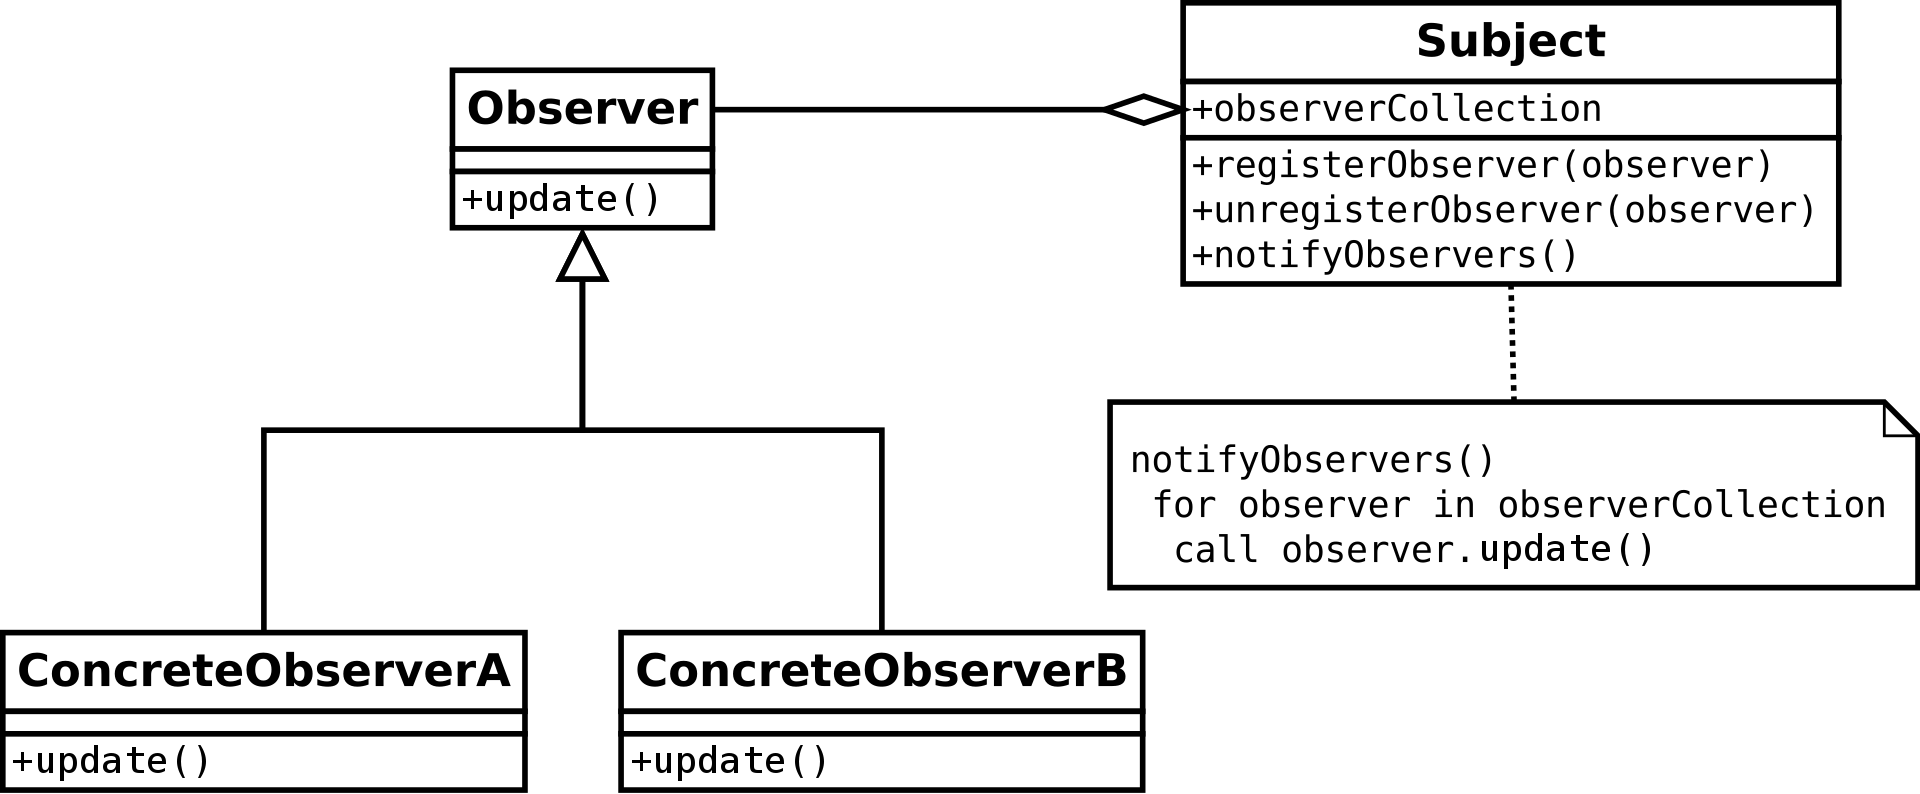
\includegraphics[width=\textwidth]{1920px-Observer_w_update.svg.png}
		\caption{Диаграмма классов UML шаблона Наблюдатель.}
	\end{center}
\end{figure}

\subsection{Пример}

Наша задача рассылать новости при появлении свежей новости на почте.
Почта - это сервис рассылки и приёма новых новостей, он и будет являться субъектом.
И есть подписчики, которые подпишутся на нашу почту и буду принимать свежие новости, они и будут являться наблюдателями.

В нашей работе есть сервер, который по-совместительству будет являться почтой, а так же есть клиенты, которые будут подписчиками.
